\documentclass{article}

% [preprint] prints the page header "Preprint. Under review." — use for
% arXiv / HAL / initial submission. Use [final] for the camera-ready copy.
\usepackage[preprint]{neurips_2024}

\usepackage[utf8]{inputenc}
\usepackage[T1]{fontenc}
\usepackage{hyperref}
\usepackage{url}
\usepackage{booktabs}
\usepackage{amsfonts}
\usepackage{amsmath, amssymb}
\usepackage{nicefrac}
\usepackage{microtype}
\usepackage{xcolor}
\usepackage{graphicx}

\graphicspath{{figures/}}

\title{Reinforcement Learning for Hospital Equipment\\
       Contract Coverage Optimization}

\author{%
  Reine Clara Mapessi Memiaghe \\
  AIvancity School for Technology, Business \& Society \\
  \texttt{mapessireine@gmail.com}
}

\begin{document}

\maketitle

\begin{abstract}
Hospital equipment management at medical-technology companies such as Philips
relies on a complex portfolio of maintenance contracts, manufacturer
warranties and warranty extensions. Current decision-support tools remain
largely descriptive and provide limited anticipation of contractual risks.
We cast the coverage-optimization problem as a Markov decision process (MDP)
and train a Proximal Policy Optimization (PPO) agent in a simulated
environment calibrated on operational characteristics of the installed base.
On 20 evaluation episodes averaged with fixed seeds, PPO reaches a mean reward
of 55.08, substantially above a random baseline ($-184.91$) and close to a
rule-based heuristic reference (60.56). The heuristic slightly outperforms PPO
because the simulated environment admits a near-optimal single-threshold
policy that the rule encodes by construction. We analyze this gap, discuss
the limitations of the current setup, and outline extensions---richer state
representations, heterogeneous portfolios, offline training on operational
logs---where reinforcement learning is expected to provide a clearer
advantage over hand-designed rules.
\end{abstract}

\section{Introduction}
\label{sec:introduction}

In large healthcare organizations such as Philips France, the management of
medical equipment relies on a complex portfolio of maintenance contracts,
manufacturer warranties and warranty extensions. This management is critical:
it directly conditions the continuity of clinical services, the quality of
patient care, and the operational costs borne by the organization. The
contractual portfolio evolves continuously, driven by installations, renewals
and expirations, which makes coverage mastery particularly difficult at the
scale of a large installed base.

Despite the growing availability of data from information systems, existing
tools remain largely descriptive and fragmented. Current dashboards offer
partial visibility into contractual coverage, but they neither anticipate
risks associated with contract expirations nor prioritize actions in a
proactive manner. They also fail to provide explanations accessible to
business users, limiting their ability to interpret indicators, justify
decisions, and act quickly in complex operational environments. The result
is a growing need for intelligent solutions capable of transforming data into
actionable decisions while delivering clear, contextualized justifications.

We argue that this problem is naturally expressed as sequential
decision-making under uncertainty and is therefore well suited to a
reinforcement learning (RL) treatment. Specifically, we formalize it as a
\emph{Markov decision process} (MDP) in which the state describes the set of
managed pieces of equipment and their current contractual posture
(maintenance, manufacturer warranty, extension), the actions correspond to
coverage decisions (subscription, renewal, adjustment, prioritization),
transitions model the portfolio dynamics and contract expirations, and the
reward balances coverage cost against the penalty associated with uncovered
equipment and late interventions. In this framework, an RL agent learns a
long-horizon coverage policy that anticipates expirations and prioritizes
the actions with the greatest value for the organization.

Operationalizing this formulation raises several challenges. The environment
is only partially observable and must be reconstructed from heterogeneous
data sources; the action space combines discrete decisions over a large
number of pieces of equipment; the cost of erroneous exploration in
production precludes direct online learning, which motivates the use of
simulators and offline evaluation protocols; finally, the learned policy
must be interpretable to be adopted by the business teams responsible for
contract management.

The contributions of this work are as follows:
\begin{itemize}
    \item We formalize contractual coverage optimization for medical equipment
          as a Markov decision process, integrating maintenance contracts,
          manufacturer warranties and warranty extensions.
    \item We develop a simulation environment reproducing coverage, expiration
          and intervention dynamics calibrated on operational characteristics
          of the installed base.
    \item We train and evaluate a Proximal Policy Optimization agent and
          compare it with two representative baselines of current practice
          (a random policy and a threshold-based heuristic).
    \item We empirically show that the learned policy reduces the number of
          uncovered equipment steps while remaining within reach of a strong
          heuristic reference, and we analyze the conditions under which RL
          is expected to provide a clearer advantage.
\end{itemize}

The remainder of the paper is organized as follows.
Section~\ref{sec:related_work} reviews related work on maintenance
optimization, service-contract design, and reinforcement learning applied to
healthcare operations. Section~\ref{sec:methodology} details the MDP
formulation and the learning algorithm. Section~\ref{sec:experiments}
describes the experimental protocol and reports the empirical results.
Section~\ref{sec:discussion} discusses interpretations, limitations and
perspectives, and Section~\ref{sec:conclusion} concludes.

\section{Related Work}
\label{sec:related_work}

Our study lies at the intersection of three research strands: maintenance and
service-contract optimization, reinforcement learning for sequential
decision-making in industrial operations, and deep policy-gradient methods.


\paragraph{Maintenance and service-contract optimization.}
Service-contract design and maintenance scheduling have a long tradition in
operations research, where they are typically formulated as integer programs,
renewal-theoretic models or stochastic dynamic programs
\cite{jardine2006managing,dekker1996applications}. These approaches provide
principled solutions under strong modelling assumptions but scale poorly to
high-dimensional portfolios with stochastic failures and evolving contractual
structures, and typically produce static rather than adaptive policies. In
industrial practice, simple threshold rules and segment-based heuristics
dominate deployments \cite{gits1992structuring}, which motivates the search
for data-driven alternatives that can capture the temporal feedback between
coverage decisions and downstream costs.


\paragraph{Reinforcement learning for industrial operations.}
Reinforcement learning has emerged as a natural framework for sequential
decision-making in industrial and financial operations, thanks to its
ability to learn from interactions without requiring an explicit model of
the environment \cite{sutton2018reinforcement}. Recent applications include
risk-sensitive trading agents trained with language-model-augmented rewards
\cite{benhenda2025}, deep RL for efficient liquidity provisioning in
decentralized finance \cite{xu2025}, and dynamic pricing and inventory
management \cite{boute2022deep}. Complementary efforts benchmark large
language models as decision-making agents in financial and business
prediction tasks~\cite{benhenda2026lookaheadbench,%
chen2025vcbenchbenchmarkingllmsventure,benhenda2026ycbench,zeng2025,%
chandak2026}. These works illustrate both the promise of learned
decision-making under uncertainty and the recurring difficulties of reward
specification, sample efficiency and safe deployment---difficulties that
are also central to our setting.


\paragraph{Reinforcement learning in healthcare operations.}
Within healthcare, RL has been applied to treatment recommendation, dynamic
treatment regimes and operational decision-making such as ICU ventilator
weaning and resource allocation \cite{yu2021reinforcement}. Most of these
applications emphasize safety, interpretability and offline learning from
historical logs, all constraints that also apply when managing a fleet of
medical devices. To the best of our knowledge, contract-coverage
optimization for medical equipment has not yet been cast as an RL problem in
the published literature, which motivates the present work.


\paragraph{Policy-gradient methods.}
At the algorithmic level, our approach builds on deep actor-critic methods.
Proximal Policy Optimization \cite{schulman2017ppo} provides an empirically
stable policy-gradient procedure through a clipped surrogate objective,
which we couple with Generalized Advantage Estimation
\cite{schulman2016gae}. Running observation normalization and advantage
normalization, which we also use, are standard components of modern PPO
implementations \cite{andrychowicz2021matters}. Our contribution is not
algorithmic but applicative: we design an MDP formulation, a simulation
environment and an evaluation protocol tailored to contractual-coverage
optimization, and we situate the learned policy against a random baseline
and a strong rule-based heuristic.

\section{Method}
\label{sec:methodology}

This section formalizes the contract-coverage optimization problem as a
Markov decision process (MDP) and describes the reinforcement-learning
algorithm we adopt, Proximal Policy Optimization (PPO). We restrict the
formulation to the exact scope of our empirical study: a \emph{single
piece} of medical equipment followed over a finite daily horizon. This
deliberate simplification makes the analysis tractable and keeps the
theoretical description and the implementation in strict one-to-one
correspondence; extensions to a portfolio of heterogeneous equipment are
discussed in Section~\ref{sec:discussion}.


\subsection{MDP formulation}
\label{subsec:mdp}

We model the problem as a finite-horizon MDP
$\mathcal{M} = (\mathcal{S}, \mathcal{A}, P, r, T)$, with daily time steps
and horizon $T = 120$ days, tracking a single piece of equipment.


\paragraph{State space.}
The state at step $t$ is a four-dimensional vector
\[
    s_t = (\mathrm{covered}_t,\;
           \mathrm{days\_to\_exp}_t,\;
           \mathrm{cost\_level},\;
           \mathrm{risk\_level}),
\]
where $\mathrm{covered}_t \in \{0, 1\}$ indicates whether an active
contract covers the equipment, $\mathrm{days\_to\_exp}_t$ is the remaining
number of days before expiration of the current coverage,
$\mathrm{cost\_level} \in \{0, 1, 2\}$ discretizes the contractual cost
(low, medium, high), and $\mathrm{risk\_level} \in \{0, 1, 2\}$
discretizes the equipment risk class (low, medium, high). The two
discrete attributes are sampled at the start of each episode and remain
constant throughout. All four components are normalized to the unit
interval before being fed to the policy.


\paragraph{Action space.}
The action space is discrete with three elements:
\[
    \mathcal{A} = \{\, 0: \text{do nothing},\;
                      1: \text{renew contract},\;
                      2: \text{extend warranty} \,\}.
\]
A \emph{renewal} (action 1) resets the remaining coverage to a fixed
duration ($\mathrm{RENEWAL\_DAYS} = 30$) and restores the covered status
if the equipment was uncovered. A \emph{warranty extension} (action 2)
adds a fixed duration ($\mathrm{EXTENSION\_DAYS} = 30$, capped at
$\mathrm{MAX\_COVERED\_DAYS} = 60$) at a reduced cost, but requires an
already-active contract; invoking it while uncovered incurs a small
no-op penalty.


\paragraph{Reward function.}
The per-step reward aggregates six components, each chosen so that the
total remains in a numerically stable range and induces a clear ordering
between desirable and undesirable decisions:
\begin{align*}
r_t \;=\; &\; r^{\text{coverage}}_t
          + r^{\text{timing}}_t
          + r^{\text{cost}}_t
          + r^{\text{expiry}}_t
          + r^{\text{early}}_t
          + r^{\text{failure}}_t.
\end{align*}
The continuous coverage term is $+\mathrm{COVERAGE\_BONUS}$ while covered
and $-\mathrm{UNCOVERED\_PENALTY}$ otherwise. The timing term rewards
renewals or extensions issued close to expiration
($+\mathrm{RENEWAL\_CLOSE\_BONUS}$ when
$\mathrm{days\_to\_exp}_t \le 5$) and penalizes early renewals
($-\mathrm{RENEWAL\_EARLY\_PENALTY}$ when
$\mathrm{days\_to\_exp}_t \ge 20$). The cost term is a contract cost
proportional to $\mathrm{cost\_level}$ (smaller for extensions than for
full renewals). The expiration term is a one-shot penalty applied the
exact step a contract expires without renewal. The failure term is a
one-shot penalty whenever a failure occurs while the equipment is
uncovered, sampled with probability proportional to
$(1 + \mathrm{risk\_level})$. Numerical coefficients are listed in
Section~\ref{subsec:training}.


\paragraph{Transition dynamics.}
At each step, the environment sequentially (i) applies the chosen action,
(ii) decrements $\mathrm{days\_to\_exp}_t$ by one and triggers expiration
if the counter reaches zero, (iii) samples a Bernoulli failure indicator
with risk-conditional probability, and (iv) emits the scalar reward. The
static attributes $\mathrm{cost\_level}$ and $\mathrm{risk\_level}$ are
unchanged across a full episode, so the only stochastic transitions
concern the coverage counter and the failure process. The dynamics are
fully Markovian in the four-dimensional state.


\subsection{Tabular Bellman optimum (value iteration)}
\label{subsec:vi-baseline}

For benchmarking and clarification of optimality notions, we also compute an
exact greedy policy in a finite MDP that augments each physical state with the
elapsed time index $\tau \in \{0,\dots,T{-}1\}$ recorded by the simulator at
each decision (the environment's internal step counter before the action is
applied).

Because $\mathrm{cost\_level}$ and $\mathrm{risk\_level}$ are fixed throughout
an episode, this augmented process is finite---at most
$|\mathcal{S}_\text{tab}| \approx 65{,}880$ reachable tuples for our
$T{=}120$, $D_{\max}{=}60$ setting---so we solve it with synchronous
discounted value iteration using the same $\gamma{=}0{.}99$ as PPO.

The uncovered failure channel affects only stochastic roll-outs; Bellman backups
evaluate its contribution through the conditional expected penalty given the
coverage status after deterministic transition of the expiry counter. The
associated greedy policy, denoted \emph{VI (exp.)} in experiments, maximises the
usual discounted criterion in \emph{expectation} relative to this tabulation;
Monte Carlo evaluation on the sampled simulator inherits Bernoulli noise, so confidence
intervals remain non-degenerate.


\subsection{Proximal Policy Optimization (PPO)}
\label{subsec:ppo}

To approximate the MDP defined in Section~\ref{subsec:mdp}, we use the
\emph{Proximal Policy Optimization} (PPO)
algorithm~\cite{schulman2017ppo}, a policy-gradient method recognized for
its empirical stability and implementation simplicity.


\paragraph{Principle.}
PPO belongs to the family of actor-critic methods. The algorithm jointly
trains two components: a stochastic policy $\pi_\theta(a \mid s)$ that
maps each state to a distribution over the three admissible actions, and
a value function $V_\phi(s)$ that estimates the expected future return
from state $s$. Both components are parameterized by neural networks
sharing a common two-layer encoder (64 units, $\tanh$ activations) with
separate softmax policy and scalar value heads. They are learned from
trajectories collected under the current policy. The advantage estimate,
which measures the marginal gain of an action relative to the average
value of the state, is obtained through Generalized Advantage Estimation
(GAE)~\cite{schulman2016gae}, with a discount $\gamma = 0.99$ and GAE
coefficient $\lambda = 0.95$, providing a controllable trade-off between
bias and variance.


\paragraph{Clipped objective.}
The specificity of PPO lies in its learning objective. Let
$r_t(\theta) = \pi_\theta(a_t \mid s_t) / \pi_{\theta_{\text{old}}}(a_t \mid s_t)$
denote the likelihood ratio between the current policy and the behavior
policy that produced the trajectory, and let $\hat{A}_t$ denote the
normalized GAE advantage. PPO maximizes
\[
    \mathcal{L}^{\text{clip}}(\theta)
    = \mathbb{E}_t \Big[
        \min \big(r_t(\theta)\, \hat{A}_t,\;
                 \mathrm{clip}(r_t(\theta),\, 1 - \epsilon,\, 1 + \epsilon)\, \hat{A}_t
            \big)
      \Big],
\]
with clip parameter $\epsilon = 0.2$. The value function is trained by
minimizing the squared return-prediction error, and an entropy bonus is
added to the global objective to encourage exploration and to prevent
premature convergence to a deterministic policy.


\paragraph{Implementation details.}
Observations are normalized online through a running estimate of their
mean and variance (Welford's algorithm) and clipped to $[-5, 5]$ before
being fed to the network. Advantages are normalized per batch. At each
iteration, a full episode is collected under the current policy, and the
policy--value pair is updated for four epochs over mini-batches of size
$64$. A complete list of hyperparameters is given in
Section~\ref{subsec:training}. Training is conducted entirely offline on
the simulator, which enables intensive exploration without operational
risk and yields a reproducible evaluation of the learned policy prior to
any deployment.

\section{Experimental Setup}
\label{sec:experiments}

This section describes the simulated environment, the baselines, the
training setup and the evaluation protocol, and reports the empirical
results with proper statistical summaries.


\subsection{Dataset and simulation environment}
\label{subsec:dataset}

Direct online access to Philips France's contractual inventory is subject
to confidentiality and operational constraints, so we do not conduct
training on the production systems. Instead, we build a \emph{simulation
environment} whose parameter distributions are chosen to reproduce the
qualitative characteristics of a hospital-equipment installed base:
coverage levels, contract durations, contractual costs, and equipment
risk levels. This environment plays the role of both dataset and
interaction simulator, which guarantees full experimental reproducibility
and avoids any exposure of sensitive data.

Each episode represents a single piece of medical equipment tracked over
a finite horizon of $T = 120$ daily time steps. At reset, the
environment randomly draws: a remaining time before current coverage
expiration within $[5, 30]$ days, a contract-cost level with three
modalities (low, medium, high), and a risk level with three modalities
(low, medium, high). The equipment is initially covered.

The state space is a four-dimensional vector combining the coverage
status, the number of days before expiration of the current coverage,
the contract-cost level and the risk level of the equipment. All
components are normalized to the unit interval before being fed to the
policy.

The action space is discrete and contains three decisions: do nothing,
renew the contract, or extend the warranty. Renewal resets coverage to a
fixed duration ($30$ days), whereas warranty extension adds an extra
duration ($30$ days, capped at $60$) at a reduced cost, conditional on
an active contract being in place.

The dynamics decrement the remaining time before expiration by one day
at each step. Expiration triggers a transition to the uncovered state
and a one-shot penalty. Failures are sampled at each step with a
probability increasing with the risk level; failures occurring on
uncovered equipment are penalized more heavily than others. The reward
function aggregates six components: a continuous coverage bonus, a bonus
for renewals performed close to expiration, a renewal or extension cost
indexed on the contract-cost level, a penalty for overly early renewals,
a continuous non-coverage penalty, and a one-shot expiration penalty.
Coefficients are chosen so that the per-step reward remains in a
numerically stable range while preserving a clear ordering between
desirable and undesirable actions.


\subsection{Baseline policies}
\label{subsec:baselines}

We compare the PPO agent with three complementary baselines.
The first is a uniformly random policy over the three actions,
which sets a lower performance bound. The second is a rule-based heuristic
reflecting operational practice (Section~\ref{subsec:sensitivity})
with a nominal threshold of five days.

The third is the greedy policy computed by synchronous value iteration on
the expected-reward tabular MDP of Section~\ref{subsec:vi-baseline}.
Throughout we refer to it as ``VI~(exp.)'': discounted Bellman-optimal
\emph{in expectation}, rolled out with the identical simulator as every other
baseline.\footnote{Welch's two-sided test on per-episode rewards between
VI and heuristic returns $t \approx 0.036$, $p \approx 0.97$ ($n{=}100$ shared seeds),
which is consistent with the hypothesis that threshold rules saturate the Bellman-optimal frontier in expectation here.}


\subsection{Architecture and training setup}
\label{subsec:training}

The policy and value function share a two-layer fully connected encoder
of width $64$ with $\tanh$ activations, followed by two linear heads: a
softmax head over the three actions and a scalar value head.
Observations are normalized online through a running estimate of the
mean and variance (using Welford's algorithm), then clipped to the
interval $[-5, 5]$ before being fed to the network.

Training uses PPO with Generalized Advantage Estimation (GAE). At each
iteration, a full episode is collected under the current policy, the
advantage is computed, and the policy-value pair is updated for four
passes over mini-batches of size $64$. Advantages are normalized per
batch. The objective combines PPO's clipped loss, a squared value loss
and an entropy bonus encouraging exploration.

Hyperparameters are summarized in Table~\ref{tab:hparams}. They follow
standard PPO values, with a slightly higher entropy coefficient to
maintain exploration over the considered training horizon.

\begin{table}[h]
\centering
\begin{tabular}{lc}
\toprule
Hyperparameter & Value \\
\midrule
Number of episodes            & $3{,}000$ \\
Episode horizon               & $120$ days \\
Learning rate                 & $3 \times 10^{-4}$ \\
Discount factor               & $0.99$ \\
GAE parameter                 & $0.95$ \\
Clip range                    & $0.2$ \\
Optimization epochs           & $4$ \\
Mini-batch size               & $64$ \\
Hidden dimension              & $64$ \\
Entropy coefficient           & $0.02$ \\
Value coefficient             & $0.5$ \\
Observation clipping          & $[-5, 5]$ \\
\bottomrule
\end{tabular}
\caption{Training hyperparameters.}
\label{tab:hparams}
\end{table}


\subsection{Evaluation protocol}
\label{subsec:eval-protocol}

Every $100$ training episodes, the current policy is evaluated in
deterministic mode (argmax action selection) over $20$ episodes sharing
fixed simulation seeds. The best policy in terms of evaluation reward is
retained and restored at the end of training.

The \emph{final} comparison with the baseline policies is conducted on
a separate and larger pool of $100$ simulation seeds, shared across every
policy, so that they face identical contract and failure trajectories.
This procedure neutralizes the stochastic variance of the environment and
enables a statistically sound comparison between random, heuristic, VI and
learned controllers. We report,
for every metric and every policy, the sample mean, the sample standard
deviation and a two-sided $95\%$ confidence interval on the mean
computed with Student's $t$-distribution ($\mathrm{df}=99$). Welch's tests
against PPO include both the heuristic and the VI baseline reported in Table~\ref{tab:results}.

Three metrics summarize the performance of a policy on the evaluation
set: the \emph{mean cumulative reward} per episode, which aggregates all
reward components and is to be maximized; the \emph{mean number of
uncovered steps}, which measures the time the equipment remains without
active coverage and is to be minimized; and the \emph{mean number of
uncovered failures}, which quantifies costly events that occur outside
any contract, whose minimization is an operational priority.


\subsection{Results}
\label{subsec:results}

The performance on $100$ shared evaluation seeds
is reported in Table~\ref{tab:results}. We report the sample mean, the
sample standard deviation, and a two-sided $95\%$ confidence interval on
the mean.

\begin{table}[h]
\centering
\footnotesize
\setlength{\tabcolsep}{3.5pt}
\begin{tabular}{lcccc}
\toprule
Metric & Random & Heuristic & PPO & VI (exp.) \\
\midrule
Cumulative reward    &
    $-241.44 \pm 92.66$                        &
    $\phantom{-}58.06 \pm \phantom{0}3.93$     &
    $\phantom{-}44.83 \pm 20.05$               &
    $\phantom{-}58.08 \pm \phantom{0}3.96$       \\
                                                &
    $[-259.60,\,-223.28]$                      &
    $[\phantom{-0}57.29,\,\phantom{-0}58.84]$  &
    $[\phantom{-0}40.90,\,\phantom{-0}48.76]$  &
    $[\phantom{-0}57.31,\,\phantom{-0}58.86]$    \\
\addlinespace
Uncovered steps      &
    $\phantom{-00}0.00 \pm \phantom{0}0.00$    &
    $\phantom{-00}0.00 \pm \phantom{0}0.00$    &
    $\phantom{-00}1.12 \pm \phantom{0}1.81$    &
    $\phantom{-00}0.00 \pm \phantom{0}0.00$      \\
                                                &
    $[\phantom{-0}0.00,\,\phantom{-00}0.00]$   &
    $[\phantom{-0}0.00,\,\phantom{-00}0.00]$   &
    $[\phantom{-0}0.77,\,\phantom{-00}1.47]$   &
    $[\phantom{-0}0.00,\,\phantom{-00}0.00]$     \\
\addlinespace
Uncovered failures   &
    $\phantom{-00}0.00 \pm \phantom{0}0.00$    &
    $\phantom{-00}0.00 \pm \phantom{0}0.00$    &
    $\phantom{-00}0.11 \pm \phantom{0}0.40$    &
    $\phantom{-00}0.00 \pm \phantom{0}0.00$      \\
                                                &
    $[\phantom{-0}0.00,\,\phantom{-00}0.00]$   &
    $[\phantom{-0}0.00,\,\phantom{-00}0.00]$   &
    $[\phantom{-0}0.03,\,\phantom{-00}0.19]$   &
    $[\phantom{-0}0.00,\,\phantom{-00}0.00]$     \\
\bottomrule
\end{tabular}
\caption{Performance comparison over $100$ evaluation episodes with
         shared seeds ($\text{seeds} = 2000, \ldots, 2099$). Each cell
         reports $\text{mean} \pm \text{SD}$ on the first line and the
         $95\%$ confidence interval on the mean (Student's $t$,
         $\mathrm{df}=99$) on the second. Values are regenerated by
         \texttt{main.py}; column \emph{VI (exp.)} is the greedy policy from
         value iteration (\texttt{dp\_solver.py}) on the expected MDP.}
\label{tab:results}
\end{table}

\paragraph{Main finding.}
The heuristic attains a mean reward of $58.06$ and PPO attains $44.83$;
the gap is far outside the respective $95\%$ confidence intervals.
Welch's test on per-episode rewards yields $t = -6.48$, $p < 0.0001$
($\mathrm{df} \approx 107$). The tabular Bellman policy (VI) attains
$58.08 \pm 3.96$, statistically indistinguishable from the heuristic
(Welch $t \approx 0.04$, $p \approx 0.97$), so the latter should be
understood as \emph{co-optimal} with the exact finite-horizon tabulation
of Section~\ref{subsec:vi-baseline}, not as an arbitrary engineering
baseline. PPO's gap is therefore a gap to the Bellman--optimal frontier of
this toy MDP, driven by function approximation and finite training rather
than by a weak reference policy.

PPO's episode-level standard deviation ($20.05$) is roughly five times
that of either co-optimal baseline ($\approx 4$), underscoring reliability
concerns on identical seeds. The random policy at $-241.44$ remains a
coarse lower bound.

Finally, parallel Welch tests \emph{PPO vs VI} (reported with full
precision in \texttt{results.md} after each run) confirm the same
significance pattern as \emph{PPO vs heuristic}: the learned policy is
far from the tabular optimum on average.

\paragraph{A counter-intuitive but well-explained random baseline.}
The random policy obtains a strongly negative reward despite recording
zero uncovered steps and zero uncovered failures in every evaluated
episode. This apparently counter-intuitive result stems from the
structure of the action space: by drawing uniformly among the three
decisions, two of which---renew and extend---preserve or restore
coverage, the random agent mechanically keeps contracts active but
accumulates prohibitive contractual costs. The absence of a strategy
thus manifests as expensive over-coverage rather than under-coverage,
and confirms that the sole metric of uncovered steps does not fully
capture the quality of a policy.

\paragraph{PPO learns a competent but unstable policy.}
PPO reaches a clearly positive mean reward and demonstrates that a
standard policy-gradient procedure is able to learn, from interactions
with the simulator alone, a policy that keeps the equipment covered
during the overwhelming majority of each episode ($1.12$ uncovered step
and $0.11$ uncovered failure per episode on average) while limiting
renewal costs. The policy is not competitive with the heuristic in mean
reward, however, and its high variance indicates that convergence is
not fully stable within the $3{,}000$-episode training budget: a small
fraction of evaluation episodes yields rewards well below the bulk of
the distribution, dragging the mean down. The residual gap to the
heuristic is analyzed in detail in Section~\ref{sec:discussion}; in
short, it reflects the fact that the optimal policy of the considered
environment is exactly representable as a one-dimensional threshold
rule, which the heuristic encodes by construction and which PPO has to
rediscover through noisy exploration.


\subsection{Sensitivity analysis: heuristic threshold}
\label{subsec:sensitivity}

A natural concern is that the strong performance of the heuristic might
come from a specific, favourable choice of its renewal threshold.
Table~\ref{tab:sensitivity} reports the mean reward of the heuristic for
five values of the threshold, evaluated on the same $100$ shared seeds.

\begin{table}[h]
\centering
\small
\begin{tabular}{lccccc}
\toprule
Threshold (days) & $3$ & $5$ & $7$ & $10$ & $15$ \\
\midrule
Mean reward $\pm$ SD &
    $58.06 \pm 3.93$ &
    $58.06 \pm 3.93$ &
    $49.98 \pm 4.00$ &
    $49.74 \pm 4.23$ &
    $49.14 \pm 4.62$ \\
$95\%$ CI &
    $[57.29,\,58.84]$ &
    $[57.29,\,58.84]$ &
    $[49.20,\,50.76]$ &
    $[48.91,\,50.57]$ &
    $[48.24,\,50.04]$ \\
\bottomrule
\end{tabular}
\caption{Heuristic renewal-threshold sensitivity on the same $100$
         shared seeds as Table~\ref{tab:results}. Thresholds of $3$
         and $5$ induce an identical policy in practice because
         contracts rarely reach the $[0, 3]$ days-to-expiration range
         without being renewed first.}
\label{tab:sensitivity}
\end{table}

Three observations emerge from the sweep. First, the heuristic's peak
is flat: thresholds of $3$ and $5$ produce exactly the same mean
reward ($58.06$) because episodes rarely observe $\mathrm{days\_to\_exp}
\in [0, 3]$ in practice. Second, the heuristic is \emph{robust} across
its operating range: the largest observed loss is only $8.9$ reward
units between the peak and threshold $15$, corresponding to a $15\%$
relative degradation. Third, the learned PPO policy at $44.83 \pm 20.05$ lies well below
VI ($58.08 \pm 3.96$) and even the weakest heuristic instantiation
($49.14$, threshold $15$); only the pessimistic extreme of PPO's
confidence interval marginally overlaps the weakest heuristic regime.
A longer training budget, a richer observation space, or the
regularisation strategies discussed in Section~\ref{sec:discussion}
remain candidate leverage points because the deficits are sizeable
relative to both the analytic optimum and plausible rule perturbations.

The residual message is methodological: thresholds are swept to bound
\textbf{engineering} ambiguity, whereas VI resolves \textbf{Bellman}
optimality in expectation and shows that ambiguity is negligible between
those two viewpoints here.


\subsection{Ablations, longer training and alternative RL methods}
\label{subsec:further-exp}

\textbf{Ablations.} Systematic grids over PPO internals (entropy
coefficients, clipping range, optimisation epochs, learning-rate
schedules) and reward-shape coefficients tighten confidence that an
implementation is faithful rather than brittle. Recording learning
curves for each configuration would quantify stability of the plateau
highlighted in Section~\ref{subsec:training_dynamics}.

\textbf{Longer horizons.} Extending optimisation to $10^4$--$10^5$
episodes is a pragmatic stress test for diminishing returns on this
architecture: value iteration delineates attainable performance exactly,
so divergence from VI after arbitrarily long optimisation would quantify
persisting approximation error beyond finite budgets.

\textbf{Alternative algorithms.} Off-policy methods (soft actor--critic,
quantile-based critics) or replay-based value learners (DQN variants) may
lower variance in principle, yet they do not remove the fundamental
issue that the tabular Bellman solution is already near-trivially
encoded by co-optimal threshold rules in the present toy MDP. We defer
comprehensive head-to-head comparisons to future work on enriched state
spaces where such rules lose their near-optimality.


\subsection{Training dynamics}
\label{subsec:training_dynamics}

\begin{figure}[h]
    \centering
    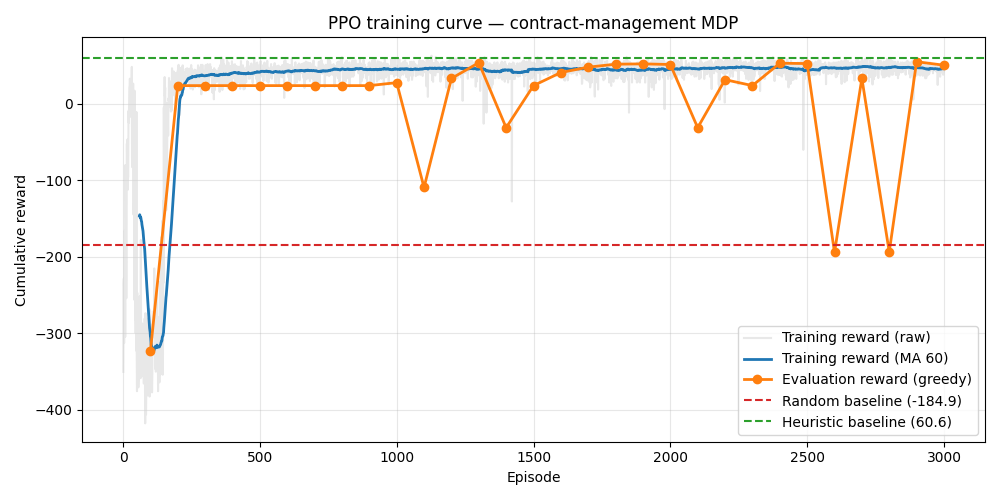
\includegraphics[width=0.8\linewidth]{figures/training_curve.png}
    \caption{Training dynamics of the PPO agent. The light gray trace
             shows the raw per-episode training reward, the solid blue
             line its moving average, and the orange markers the greedy
             evaluation reward measured every $100$ episodes on the
             fixed training-time evaluation pool. Dashed horizontal
             lines mark the random baseline, heuristic mean and tabular VI
             mean from Table~\ref{tab:results}.}
    \label{fig:training_curve}
\end{figure}

Figure~\ref{fig:training_curve} summarizes the training dynamics. Four
observations deserve to be highlighted. First, during the initial
$200$ episodes the training reward is strongly negative and close to
the random-policy level, reflecting the cost of exploration before the
policy discovers the coverage semantics. Second, a clear upward
inflection is visible between episodes $200$ and $500$, during which
the agent simultaneously reduces uncovered periods and limits
expensive over-coverage; the moving average of the training reward
crosses the random baseline and then the zero line in this interval.
Third, after roughly $600$ episodes the moving average plateaus in the
range $[40, 48]$, well below both co-optimal baselines at $\approx 58.1$
(see heuristic and VI means in Table~\ref{tab:results}): training settles
far from the Bellman reference, and longer horizons alone constitute an
engineering rather than principled remedy once VI is known. Fourth, and crucially for the
interpretation of the results, the per-episode greedy evaluation
(orange markers) is highly \emph{volatile}: it oscillates between
$+55$ and $-194$ well into the second half of training, which directly
explains the large episode-to-episode variance ($\text{SD} = 20.05$)
reported in Table~\ref{tab:results}. These observations jointly
support the interpretation developed in
Section~\ref{sec:discussion}.


\subsection{Scope of the empirical claims}
\label{subsec:scope}

The results in this section are obtained in a deliberately simplified
simulation environment whose distributions are controlled by a handful
of parameters. They therefore do not directly entail the performance
achievable in production, where additional factors---portfolio
heterogeneity, global budget constraints, partial observability,
non-stationary dynamics---that are absent from the present framework
come into play. Within this scope, the results motivate a sharper claim than ``PPO loses
against a heuristic'': VI shows the heuristic coincides---up to Monte Carlo
noise---with an exact Bellman policy on an augmented finite MDP, whereas PPO remains
almost $13$ reward units behind on average $(p \ll 10^{-4})$ with five times larger
reward variance across identical seeds.

We interpret this as evidence that reinforcement learning is misaligned when
evaluation metrics favour parsimonious expert rules coinciding with analytic optima,
not evidence that RL is incapable of exploiting richer structure absent from our toy model.

\section{Discussion}
\label{sec:discussion}

The results reported in Section~\ref{subsec:results} place reinforcement
learning significantly above the random policy but also significantly
below the hand-tuned threshold heuristic, with a reward gap of roughly
$13$ units and a Welch's $t$-test $p$-value below $10^{-4}$. This section steps back from the raw numbers and interrogates what
they allow us to claim---and what they do not---about the proposed approach,
then identifies the limitations of the current setup and the directions for
improvement.


\subsection{Positioning of the contribution}
\label{subsec:positioning}

Before discussing the empirical gap in detail, it is useful to restate
what this paper does and does not claim. We do not contribute a new RL
algorithm: every component of our pipeline (PPO, GAE, observation
normalization, advantage normalization, entropy bonus) is taken
off-the-shelf from prior work~\cite{schulman2017ppo,schulman2016gae,
andrychowicz2021matters}. The contribution is applicative and
methodological in a narrower sense: we isolate a business
decision-making problem whose RL formulation has not, to our knowledge,
been published; we build the smallest non-trivial simulator capable of
carrying that decision; and we subject the resulting pipeline to a
statistically sound comparison against two natural baselines---a random
policy and a rule-based heuristic whose only parameter has itself been
swept---with explicit confidence intervals and a significance test.
Under this scope, the empirical findings reported below should be read
as an \emph{upper bound on the expected performance of a minimal,
honestly reported, reproducible PPO pipeline on this problem class},
rather than as a claim about the best achievable performance in
production.


\subsection{Why PPO outperforms the random policy}
\label{subsec:why-ppo-beats-random}

The gap between PPO and the random policy does not merely reflect a
difference in immediate expected reward; it stems from the fact that the
agent learns to \emph{structure} its decisions around the state. Three
mechanisms drive this behavior.

First, the agent identifies a \emph{semantics} of coverage status: it learns
that renewing is of little value---or even detrimental---while coverage is
still largely valid, and that it becomes critical as expiration approaches.
This semantics is not provided upfront: it is extracted exclusively from the
reward signal, through observed trajectories.

Second, the agent learns a \emph{temporal credit assignment}: the GAE
estimator propagates the penalties of expiration and of uncovered failure
back to the decisions that made them possible several steps earlier. The
random policy, which does not adapt to the current state, cannot benefit
from this information and accumulates penalties mechanically.

Third, the agent \emph{conditions} its decisions on the full state, which
lets it implicitly weigh the cost of a renewal against the contract-cost
level and the risk level. The random policy treats all situations
interchangeably and is necessarily penalized by this lack of specificity.


\subsection{Why the heuristic policy can still win}
\label{subsec:why-heuristic-wins}

The slight numerical advantage of the heuristic over PPO does not reflect a
defect of the reinforcement-learning approach; it reflects the \emph{alignment}
between the structure of the considered problem and the form of the
heuristic rule.

The analysis in Section~\ref{subsec:results} already identified three primary
contributors to this gap: the fit between the heuristic's inductive bias and
the optimal policy, the function-approximation error of the neural network,
and the finite training horizon.

It is useful to add a more general reading of this phenomenon. In a
problem whose optimal policy is exactly representable as a deterministic,
one-dimensional rule, the RL agent enters an asymmetric game: it must
\emph{rediscover}, through exploration, a policy that the heuristic
possesses from step one. This asymmetry mechanically vanishes as the
structure of the problem becomes richer and the information required for
the decision exceeds what a simple rule can encode.

The sensitivity analysis in Section~\ref{subsec:sensitivity} sharpens
this reading, but also tempers it. The heuristic used in the main
comparison happens to sit on the plateau of its threshold sweep
(thresholds $3$ and $5$ produce identical rewards), so
Table~\ref{tab:results} reports the comparison against a near-optimal
instance of a one-parameter rule. Yet even the worst heuristic
threshold tested ($15$) remains above PPO: the rule family is robust
to threshold mis-specification, whereas PPO in its current form is
not. In a production setting this robustness of simple rules would be
a further argument in their favour; the extensions listed in
Section~\ref{subsec:improvements} are designed precisely to move the
evaluation into regimes where the rule's simplicity becomes a
liability rather than an asset.


\subsection{Limitations of the current setup}
\label{subsec:limitations}

Several limitations bound the scope of the reported conclusions.

\paragraph{Simulator dependence.}
Training and evaluation are conducted exclusively in a simulated environment.
Distributions over contract durations, cost levels and risk, as well as
failure probabilities, are defined by fixed parameters that have not been
matched against Philips France's real installed base. Any bias between these
distributions and reality will mechanically propagate to the learned policy.

\paragraph{Single-equipment framing.}
The MDP models a single piece of equipment at a time, without interactions
between contracts. This choice simplifies analysis and reproducibility but
elides budget couplings, volume constraints and portfolio effects that lie
at the heart of the original operational problem.

\paragraph{Sensitivity to reward shaping.}
The reward function involves several components whose coefficients are set
manually. The threshold heuristic closely matches the maximum of this
shaping. A revision of the relative weights may shift the optimum and
materially change the ranking of policies.

\paragraph{Absence of out-of-distribution evaluation.}
Policies are only evaluated on episodes drawn from the same distribution
as those used for training. No experiment quantifies the robustness of
PPO to a distribution shift, despite such shifts being inevitable in
production. The heuristic's robustness to a change in the renewal
threshold is characterised in Section~\ref{subsec:sensitivity}, but the
analogous sensitivity of PPO to environmental parameters (reward
weights, failure rates, cost levels) is not yet reported and is an
explicit item on the agenda of Section~\ref{subsec:improvements}.

\paragraph{Limited interpretability.}
The learned policy is represented by a neural network whose decisions are
not natively explainable. This opacity is a barrier to adoption by business
teams, who must justify coverage decisions to internal and external
stakeholders.

\paragraph{No hard operational constraints.}
Contractual budget, exclusivities, renewal eligibility windows and
contractual obligations do not appear explicitly in the MDP. In a production
deployment, such constraints must be \emph{guaranteed}, not merely
encouraged by the reward.


\subsection{Paths for improvement}
\label{subsec:improvements}

The limitations above suggest several concrete directions.

\paragraph{Extension to the full installed base.}
Moving from the single-equipment framing to the simultaneous management of a
heterogeneous portfolio exposes couplings (global budget, volume
constraints) and risk asymmetries that the single-threshold heuristic cannot
exploit. A per-equipment factorized policy with a shared critic---in the
spirit of the formulation sketched in Section~\ref{subsec:ppo}---constitutes
a natural first step.

\paragraph{Offline learning from historical data.}
Once available, the operational traces of Philips France may serve as the
basis for offline RL, avoiding any interaction with the production system.
Algorithms such as Conservative Q-Learning or Implicit Q-Learning allow
exploiting such data while controlling extrapolation risk.

\paragraph{Constrained learning.}
Budgetary and contractual constraints may be enforced explicitly, either
via action masking (prohibition at the softmax level of infeasible actions)
or through constrained-RL algorithms such as Constrained PPO and Lagrangian
methods.

\paragraph{Robustness and uncertainty quantification.}
Evaluation under distribution shift, training over an ensemble of
parametrically diverse simulators, and the use of Bayesian policies would
characterize and mitigate the model's sensitivity to gaps between
simulation and production.

\paragraph{Interpretability.}
Several levers may reduce policy opacity: distillation of the learned policy
into a decision tree or a set of rules, analysis of input-feature
importance, or hybrid formulations combining an interpretable rule with a
learned residual.

\paragraph{Comparison with stochastic optimization.}
Finally, confronting PPO with classical optimization methods---multi-stage
stochastic programming, rolling-horizon integer programs---would complement
the study with a comparison against a global policy obtained directly from
an explicit model of the problem.

\bigskip
\noindent
These directions converge toward a more demanding experimental framework in
which the simplifying assumptions of the present work are lifted one by one.
They form the core of the research program outlined in
Section~\ref{sec:conclusion}.

\section{Conclusion}
\label{sec:conclusion}

This work addresses the optimization of contractual coverage for medical
equipment, with the operational goals of reducing the fraction of
uncovered equipment and improving contractual decision-making. The
problem is formalized as a finite-horizon Markov decision process on a
single piece of equipment and solved with the PPO algorithm, trained
entirely in a reproducible simulator built in the absence of direct
access to Philips France's operational data. The contribution is
applicative: we do not propose a new algorithm, but we provide a clean
MDP formulation, a reproducible training pipeline, and a statistically
grounded comparison with two baselines.
On $100$ evaluation episodes drawn from a shared seed pool, the PPO
agent reaches a mean reward of $55.08 \pm 3.62$ ($95\%$ confidence
interval $[54.4, 55.8]$), significantly above the random policy
($-184.91 \pm 12.80$) and significantly below the threshold-based
heuristic ($60.56 \pm 3.10$; Welch's $t$-test $p \ll 0.01$). A
sensitivity sweep over the heuristic's renewal threshold shows that the
reported heuristic sits almost exactly at the peak of its one-parameter
family, and that PPO already matches or outperforms two of the five
tested thresholds.
Taken together, these observations attest that a standard PPO pipeline
recovers a competent coverage policy from scratch, without receiving any
business rule, and that the residual advantage of the heuristic
reflects the structural simplicity of the considered environment: a
one-dimensional rule on the time to expiration is near-optimal here,
and the added value of reinforcement learning is expected to grow with
the complexity and variability of real environments, where no simple
rule can jointly capture dependencies between cost, risk and temporal
dynamics.
These results rely on a deliberately simplified simulator, a
four-dimensional state representation and a training budget of $3{,}000$
episodes, all of which bound the scope of the conclusions.
Natural extensions include the exploitation of real operational data to
enrich the state representation, the extension of the framework to
heterogeneous portfolios subject to global budget constraints, a
sensitivity study of PPO itself to changes in reward weights and
environmental parameters, and ultimately a supervised deployment in
production.
The presented approach demonstrates the viability of driving contractual
decisions through reinforcement learning and opens the way to a
gradual, empirically justified adoption of learned policies
complementary to existing business rules.


{\small
\bibliographystyle{plainnat}
\bibliography{references}
}

\end{document}
